%%*************************************************************************
%% Legal Notice:
%% This code is offered as-is without any warranty either expressed or
%% implied; without even the implied warranty of MERCHANTABILITY or
%% FITNESS FOR A PARTICULAR PURPOSE! 
%% User assumes all risk.
%% In no event shall IEEE or any contributor to this code be liable for
%% any damages or losses, including, but not limited to, incidental,
%% consequential, or any other damages, resulting from the use or misuse
%% of any information contained here.
%%
%% All comments are the opinions of their respective authors and are not
%% necessarily endorsed by the IEEE.
%%
%% This work is distributed under the LaTeX Project Public License (LPPL)
%% ( http://www.latex-project.org/ ) version 1.3, and may be freely used,
%% distributed and modified. A copy of the LPPL, version 1.3, is included
%% in the base LaTeX documentation of all distributions of LaTeX released
%% 2003/12/01 or later.
%% Retain all contribution notices and credits.
%% ** Modified files should be clearly indicated as such, including  **
%% ** renaming them and changing author support contact information. **
%%
%% File list of work: IEEEtran.cls, IEEEtran_HOWTO.pdf, bare_adv.tex,
%%                    bare_conf.tex, bare_jrnl.tex, bare_jrnl_compsoc.tex
%%*************************************************************************

% *** Authors should verify (and, if needed, correct) their LaTeX system  ***
% *** with the testflow diagnostic prior to trusting their LaTeX platform ***
% *** with production work. IEEE's font choices can trigger bugs that do  ***
% *** not appear when using other class files.                            ***
% The testflow support page is at:
% http://www.michaelshell.org/tex/testflow/



% Note that the a4paper option is mainly intended so that authors in
% countries using A4 can easily print to A4 and see how their papers will
% look in print - the typesetting of the document will not typically be
% affected with changes in paper size (but the bottom and side margins will).
% Use the testflow package mentioned above to verify correct handling of
% both paper sizes by the user's LaTeX system.
%
% Also note that the "draftcls" or "draftclsnofoot", not "draft", option
% should be used if it is desired that the figures are to be displayed in
% draft mode.
%
\documentclass[conference]{IEEEtran}
% Add the compsoc option for Computer Society conferences.
%
% If IEEEtran.cls has not been installed into the LaTeX system files,
% manually specify the path to it like:
% \documentclass[conference]{../sty/IEEEtran}





% Some very useful LaTeX packages include:
% (uncomment the ones you want to load)


% *** MISC UTILITY PACKAGES ***
%
%\usepackage{ifpdf}
% Heiko Oberdiek's ifpdf.sty is very useful if you need conditional
% compilation based on whether the output is pdf or dvi.
% usage:
% \ifpdf
%   % pdf code
% \else
%   % dvi code
% \fi
% The latest version of ifpdf.sty can be obtained from:
% http://www.ctan.org/tex-archive/macros/latex/contrib/oberdiek/
% Also, note that IEEEtran.cls V1.7 and later provides a builtin
% \ifCLASSINFOpdf conditional that works the same way.
% When switching from latex to pdflatex and vice-versa, the compiler may
% have to be run twice to clear warning/error messages.






% *** CITATION PACKAGES ***
%
%\usepackage{cite}
% cite.sty was written by Donald Arseneau
% V1.6 and later of IEEEtran pre-defines the format of the cite.sty package
% \cite{} output to follow that of IEEE. Loading the cite package will
% result in citation numbers being automatically sorted and properly
% "compressed/ranged". e.g., [1], [9], [2], [7], [5], [6] without using
% cite.sty will become [1], [2], [5]--[7], [9] using cite.sty. cite.sty's
% \cite will automatically add leading space, if needed. Use cite.sty's
% noadjust option (cite.sty V3.8 and later) if you want to turn this off.
% cite.sty is already installed on most LaTeX systems. Be sure and use
% version 4.0 (2003-05-27) and later if using hyperref.sty. cite.sty does
% not currently provide for hyperlinked citations.
% The latest version can be obtained at:
% http://www.ctan.org/tex-archive/macros/latex/contrib/cite/
% The documentation is contained in the cite.sty file itself.






% *** GRAPHICS RELATED PACKAGES ***
%
\ifCLASSINFOpdf
\usepackage[pdftex]{graphicx}
  % declare the path(s) where your graphic files are
\graphicspath{{./images/}}
  % and their extensions so you won't have to specify these with
  % every instance of \includegraphics
\DeclareGraphicsExtensions{.jpg,.png}
\else
  % or other class option (dvipsone, dvipdf, if not using dvips). graphicx
  % will default to the driver specified in the system graphics.cfg if no
  % driver is specified.
  % \usepackage[dvips]{graphicx}
  % declare the path(s) where your graphic files are
  % \graphicspath{{../eps/}}
  % and their extensions so you won't have to specify these with
  % every instance of \includegraphics
  % \DeclareGraphicsExtensions{.eps}
\fi
% graphicx was written by David Carlisle and Sebastian Rahtz. It is
% required if you want graphics, photos, etc. graphicx.sty is already
% installed on most LaTeX systems. The latest version and documentation can
% be obtained at: 
% http://www.ctan.org/tex-archive/macros/latex/required/graphics/
% Another good source of documentation is "Using Imported Graphics in
% LaTeX2e" by Keith Reckdahl which can be found as epslatex.ps or
% epslatex.pdf at: http://www.ctan.org/tex-archive/info/
%
% latex, and pdflatex in dvi mode, support graphics in encapsulated
% postscript (.eps) format. pdflatex in pdf mode supports graphics
% in .pdf, .jpeg, .png and .mps (metapost) formats. Users should ensure
% that all non-photo figures use a vector format (.eps, .pdf, .mps) and
% not a bitmapped formats (.jpeg, .png). IEEE frowns on bitmapped formats
% which can result in "jaggedy"/blurry rendering of lines and letters as
% well as large increases in file sizes.
%
% You can find documentation about the pdfTeX application at:
% http://www.tug.org/applications/pdftex





% *** MATH PACKAGES ***
%
%\usepackage[cmex10]{amsmath}
% A popular package from the American Mathematical Society that provides
% many useful and powerful commands for dealing with mathematics. If using
% it, be sure to load this package with the cmex10 option to ensure that
% only type 1 fonts will utilized at all point sizes. Without this option,
% it is possible that some math symbols, particularly those within
% footnotes, will be rendered in bitmap form which will result in a
% document that can not be IEEE Xplore compliant!
%
% Also, note that the amsmath package sets \interdisplaylinepenalty to 10000
% thus preventing page breaks from occurring within multiline equations. Use:
%\interdisplaylinepenalty=2500
% after loading amsmath to restore such page breaks as IEEEtran.cls normally
% does. amsmath.sty is already installed on most LaTeX systems. The latest
% version and documentation can be obtained at:
% http://www.ctan.org/tex-archive/macros/latex/required/amslatex/math/





% *** SPECIALIZED LIST PACKAGES ***
%
%\usepackage{algorithmic}
% algorithmic.sty was written by Peter Williams and Rogerio Brito.
% This package provides an algorithmic environment fo describing algorithms.
% You can use the algorithmic environment in-text or within a figure
% environment to provide for a floating algorithm. Do NOT use the algorithm
% floating environment provided by algorithm.sty (by the same authors) or
% algorithm2e.sty (by Christophe Fiorio) as IEEE does not use dedicated
% algorithm float types and packages that provide these will not provide
% correct IEEE style captions. The latest version and documentation of
% algorithmic.sty can be obtained at:
% http://www.ctan.org/tex-archive/macros/latex/contrib/algorithms/
% There is also a support site at:
% http://algorithms.berlios.de/index.html
% Also of interest may be the (relatively newer and more customizable)
% algorithmicx.sty package by Szasz Janos:
% http://www.ctan.org/tex-archive/macros/latex/contrib/algorithmicx/




% *** ALIGNMENT PACKAGES ***
%
%\usepackage{array}
% Frank Mittelbach's and David Carlisle's array.sty patches and improves
% the standard LaTeX2e array and tabular environments to provide better
% appearance and additional user controls. As the default LaTeX2e table
% generation code is lacking to the point of almost being broken with
% respect to the quality of the end results, all users are strongly
% advised to use an enhanced (at the very least that provided by array.sty)
% set of table tools. array.sty is already installed on most systems. The
% latest version and documentation can be obtained at:
% http://www.ctan.org/tex-archive/macros/latex/required/tools/


%\usepackage{mdwmath}
%\usepackage{mdwtab}
% Also highly recommended is Mark Wooding's extremely powerful MDW tools,
% especially mdwmath.sty and mdwtab.sty which are used to format equations
% and tables, respectively. The MDWtools set is already installed on most
% LaTeX systems. The lastest version and documentation is available at:
% http://www.ctan.org/tex-archive/macros/latex/contrib/mdwtools/


% IEEEtran contains the IEEEeqnarray family of commands that can be used to
% generate multiline equations as well as matrices, tables, etc., of high
% quality.


%\usepackage{eqparbox}
% Also of notable interest is Scott Pakin's eqparbox package for creating
% (automatically sized) equal width boxes - aka "natural width parboxes".
% Available at:
% http://www.ctan.org/tex-archive/macros/latex/contrib/eqparbox/





% *** SUBFIGURE PACKAGES ***
%\usepackage[tight,footnotesize]{subfigure}
% subfigure.sty was written by Steven Douglas Cochran. This package makes it
% easy to put subfigures in your figures. e.g., "Figure 1a and 1b". For IEEE
% work, it is a good idea to load it with the tight package option to reduce
% the amount of white space around the subfigures. subfigure.sty is already
% installed on most LaTeX systems. The latest version and documentation can
% be obtained at:
% http://www.ctan.org/tex-archive/obsolete/macros/latex/contrib/subfigure/
% subfigure.sty has been superceeded by subfig.sty.



%\usepackage[caption=false]{caption}
%\usepackage[font=footnotesize]{subfig}
% subfig.sty, also written by Steven Douglas Cochran, is the modern
% replacement for subfigure.sty. However, subfig.sty requires and
% automatically loads Axel Sommerfeldt's caption.sty which will override
% IEEEtran.cls handling of captions and this will result in nonIEEE style
% figure/table captions. To prevent this problem, be sure and preload
% caption.sty with its "caption=false" package option. This is will preserve
% IEEEtran.cls handing of captions. Version 1.3 (2005/06/28) and later 
% (recommended due to many improvements over 1.2) of subfig.sty supports
% the caption=false option directly:
%\usepackage[caption=false,font=footnotesize]{subfig}
%
% The latest version and documentation can be obtained at:
% http://www.ctan.org/tex-archive/macros/latex/contrib/subfig/
% The latest version and documentation of caption.sty can be obtained at:
% http://www.ctan.org/tex-archive/macros/latex/contrib/caption/




% *** FLOAT PACKAGES ***
%
%\usepackage{fixltx2e}
% fixltx2e, the successor to the earlier fix2col.sty, was written by
% Frank Mittelbach and David Carlisle. This package corrects a few problems
% in the LaTeX2e kernel, the most notable of which is that in current
% LaTeX2e releases, the ordering of single and double column floats is not
% guaranteed to be preserved. Thus, an unpatched LaTeX2e can allow a
% single column figure to be placed prior to an earlier double column
% figure. The latest version and documentation can be found at:
% http://www.ctan.org/tex-archive/macros/latex/base/



\usepackage{stfloats}
% stfloats.sty was written by Sigitas Tolusis. This package gives LaTeX2e
% the ability to do double column floats at the bottom of the page as well
% as the top. (e.g., "\begin{figure*}[!b]" is not normally possible in
% LaTeX2e). It also provides a command:
%\fnbelowfloat
% to enable the placement of footnotes below bottom floats (the standard
% LaTeX2e kernel puts them above bottom floats). This is an invasive package
% which rewrites many portions of the LaTeX2e float routines. It may not work
% with other packages that modify the LaTeX2e float routines. The latest
% version and documentation can be obtained at:
% http://www.ctan.org/tex-archive/macros/latex/contrib/sttools/
% Documentation is contained in the stfloats.sty comments as well as in the
% presfull.pdf file. Do not use the stfloats baselinefloat ability as IEEE
% does not allow \baselineskip to stretch. Authors submitting work to the
% IEEE should note that IEEE rarely uses double column equations and
% that authors should try to avoid such use. Do not be tempted to use the
% cuted.sty or midfloat.sty packages (also by Sigitas Tolusis) as IEEE does
% not format its papers in such ways.





% *** PDF, URL AND HYPERLINK PACKAGES ***
%
%\usepackage{url}
% url.sty was written by Donald Arseneau. It provides better support for
% handling and breaking URLs. url.sty is already installed on most LaTeX
% systems. The latest version can be obtained at:
% http://www.ctan.org/tex-archive/macros/latex/contrib/misc/
% Read the url.sty source comments for usage information. Basically,
% \url{my_url_here}.





% *** Do not adjust lengths that control margins, column widths, etc. ***
% *** Do not use packages that alter fonts (such as pslatex).         ***
% There should be no need to do such things with IEEEtran.cls V1.6 and later.
% (Unless specifically asked to do so by the journal or conference you plan
% to submit to, of course. )


% correct bad hyphenation here
\hyphenation{op-tical net-works semi-conduc-tor}


\begin{document}
%
% paper title
% can use linebreaks \\ within to get better formatting as desired
\title{A Blocks-Based Editor for HTML Code}

% author names and affiliations
% use a multiple column layout for up to three different
% affiliations
\author{
\IEEEauthorblockN{Saksham Aggarwal}
\and
\IEEEauthorblockN{David Anthony Bau}
\IEEEauthorblockA{Phillips Exeter Academy\\
Exeter, New Hampshire 03833\\
Email: dbau@exeter.edu}
}

% conference papers do not typically use \thanks and this command
% is locked out in conference mode. If really needed, such as for
% the acknowledgment of grants, issue a \IEEEoverridecommandlockouts
% after \documentclass

% for over three affiliations, or if they all won't fit within the width
% of the page, use this alternative format:
% 
%\author{\IEEEauthorblockN{Michael Shell\IEEEauthorrefmark{1},
%Homer Simpson\IEEEauthorrefmark{2},
%James Kirk\IEEEauthorrefmark{3}, 
%Montgomery Scott\IEEEauthorrefmark{3} and
%Eldon Tyrell\IEEEauthorrefmark{4}}
%\IEEEauthorblockA{\IEEEauthorrefmark{1}School of Electrical and Computer Engineering\\
%Georgia Institute of Technology,
%Atlanta, Georgia 30332--0250\\ Email: see http://www.michaelshell.org/contact.html}
%\IEEEauthorblockA{\IEEEauthorrefmark{2}Twentieth Century Fox, Springfield, USA\\
%Email: homer@thesimpsons.com}
%\IEEEauthorblockA{\IEEEauthorrefmark{3}Starfleet Academy, San Francisco, California 96678-2391\\
%Telephone: (800) 555--1212, Fax: (888) 555--1212}
%\IEEEauthorblockA{\IEEEauthorrefmark{4}Tyrell Inc., 123 Replicant Street, Los Angeles, California 90210--4321}}




% use for special paper notices
%\IEEEspecialpapernotice{(Invited Paper)}




% make the title area
\maketitle


\begin{abstract}
%\boldmath
  Droplet is a new dual-mode editor that allows students to work in either blocks or text and switch between them any time. This paper presents work creating a Droplet mode for HTML code. We also discuss an analysis of real-world HTML tags and attributes and propose a palette based on this analysis.

\end{abstract}
% IEEEtran.cls defaults to using nonbold math in the Abstract.
% This preserves the distinction between vectors and scalars. However,
% if the conference you are submitting to favors bold math in the abstract,
% then you can use LaTeX's standard command \boldmath at the very start
% of the abstract to achieve this. Many IEEE journals/conferences frown on
% math in the abstract anyway.

% no keywords




% For peer review papers, you can put extra information on the cover
% page as needed:
% \ifCLASSOPTIONpeerreview
% \begin{center} \bfseries EDICS Category: 3-BBND \end{center}
% \fi
%
% For peerreview papers, this IEEEtran command inserts a page break and
% creates the second title. It will be ignored for other modes.
\IEEEpeerreviewmaketitle

\section{Introduction}
Teaching HTML has long been an early step in a programming curriculum.  For example Budny, et al \cite{Budny} in Four Steps to Teaching C Programming, suggest "The layout of a web page allowed us to begin to teach the basic concepts of program layout... We are teaching web page design ... not for the purpose of teaching HTML, but to teach students the concept of writing code." Mahmoud, et al \cite{Mahmoud} suggest that starting with HTML is a way of teaching "programming for fun" and is a strategy for motivating students.

Nonetheless, for first-time-coder, HTML can be difficult to learn.  In a workshop with English students, Mauriello, Pagnucci, and Winner \cite{Mauriello} observed "Students are generally not careful and experienced enough in their reading of the codes to find mistakes."  For non-coding students, Taylor and Gitsaki \cite{Taylor} suggest simplifying the problem by starting with a small set of about 30 HTML tags to create a basic web page.

Therefore we are interested in finding an alternative to WYSIWYG HTML tools that expose the code, while still simplifying the process of learning to use HTML tags for the first time.  In recent years, block programming languages such as Scratch \cite{Scratch} have introduced many students to coding through a visual representation of commands and control flow.  Here we investigate whether a similar approach can be effective when used with HTML code.

\subsection{Droplet's Text-First Approach to Blocks}

\begin{figure*}
\centering
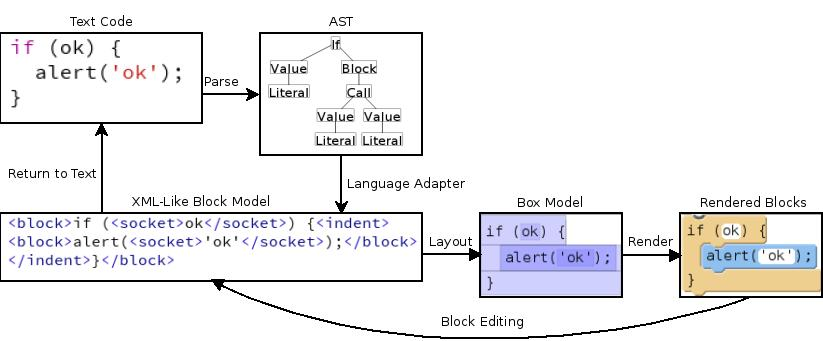
\includegraphics[width=5in]{image11.jpg}
\caption{Lifecycle of a Droplet Program}
\label{lifecycle}
\end{figure*}

Droplet \cite{Droplet} is a dual-mode blocks and text editor that was built to bridge the gap between blocks and text. Droplet's primary guiding philosophy is that the text, not the blocks, are the primary data. Thus, Droplet programs begin and end their life as text. When Droplet opens a program file, the language adapter inserts markup indicating where blocks should go and how they should be rendered. The user interacts with this rendering of the program, performing splice operations on the markup stream. During editing, the language mode may be called back to preserve precedence or dictate droppability rules. At the end of the editing session, the markup is simply discarded and a raw text program is generated again. Figure \ref{lifecycle} shows a typical Droplet editing session in JavaScript.

\subsection{Adding A New Language to Droplet}

A Droplet language adapter has two roles: to parse text and insert block markup, and to enforce droppability rules between blocks and sockets. Usually, a Droplet language adapter uses a standard language parser -- for instance, Droplet's JavaScript mode uses acorn.js -- and inserts blocks using the location data from the generated AST. The parser annotates the generated blocks with information pertinent to droppability, and uses this information later during editing to determine whether a drop is legal.

\section{Process}

\subsection{Adapting A Parser}
One of the goals of an HTML mode in Droplet is to be able to visualize existing webpages from the Internet as blocks. This poses a difficulty because browsers are tolerant and many existing webpages are not standards-compliant or are syntactically incorrect. Droplet's HTML mode adapts the parse5 \cite{parse5} HTML parser, which tolerates syntactically incorrect HTML code in the same way browsers do. The parse5 parser was modified for Droplet's purposes to add more detailed location data.

\subsection{Enforcing Droppability Rules}
One major advantage of a block language, however, is that it can enforce creating only standards-compliant code. Droplet's HTML mode therefore enforces droppability rules adapted from the WHATWG HTML specifications \cite{WHATWG}.

\subsection{Choosing A Palette}

According to Whoever \cite{Whoever}, the palette in a block language is important to discovery and self-directed learning, because students can try new commands without having to read documentation. Having a palette that contains useful and rewarding tags in an HTML mode is therefore important. The WHATWG HTML specifications define over 100 tags, however, most of which are not used. A number of developers online have informally posted HTML cheat sheets with the "most important tags," \cite{CheatSheet1} \cite{CheatSheet2} \cite{CheatSheet3} but these are subjective and often conflict with each other. Because Droplet's philosophy is to be able to interact with real-world code on the Internet, we here determine and recommend a palette based on real-world tag frequencies.

\begin{figure*}
\centering
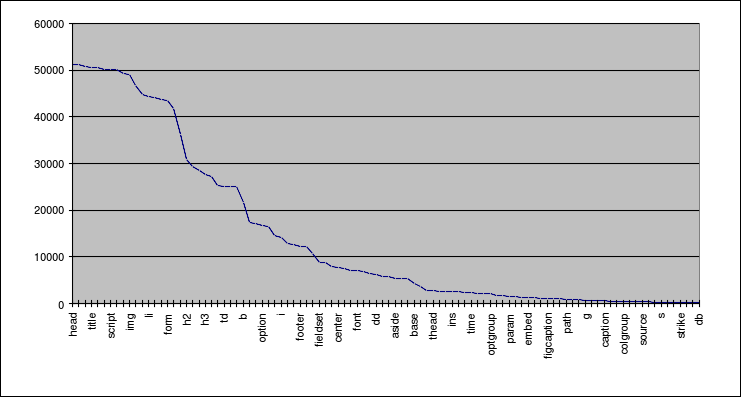
\includegraphics[width=5in]{image03.png}
\caption{Counts Based On Tag Appearances}
\label{TagsTotal}
\end{figure*}

\begin{figure*}
\centering
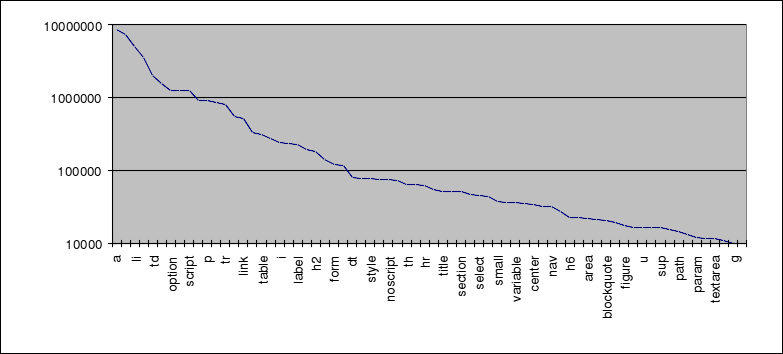
\includegraphics[width=5in]{image02.png}
\caption{Counts Based on Documents With Tag}
\label{TagsPerDocument}
\end{figure*}

Figures \ref{TagsTotal} and \ref{TagsPerDocument} show an analysis of tag frequencies over random HTML datasets collected from commoncrawl \cite{commoncrawl} (data and full results are available on Github \cite{FullResults}.  Figure \ref{TagsTotal} represents a count of the number of times each tag was used at all in the crawled data sets. Figure \ref{TagsPerDocument} represents a count of the number of documents in the data sets that used the tag.

\begin{thebibliography}{1}

\bibitem{Droplet}
  Bau, D. A. Droplet, A Blocks-Based Editor for Text Code. Journal of Computer Science in Colleges. 30, 6 (June 2015).
\bibitem{Budny}
  Budny, D.; Lund, L.; Vipperman, J.; Patzer, J.L.I.I.I., "Four steps to teaching C programming," Frontiers in Education, 2002. FIE 2002. 32nd Annual , vol.2, no., pp.F1G-18,F1G-22 vol.2, 2002
\bibitem{Mahmoud}
  Qusay H. Mahmoud, Wlodek Dobosiewicz, and David Swayne. 2004. Redesigning introductory computer programming with HTML, JavaScript, and Java. SIGCSE Bull. 36, 1 (March 2004), 120-124. DOI=10.1145/1028174.971344 http://doi.acm.org/10.1145/1028174.971344
\bibitem{Mauriello}
  Mauriello, N. Pagnucci, G. and Winner, T. Reading between the Code: The Teaching of HTML and the Displacement of Writing Instruction. Computers and Composition 16, 409-19 (1999)
\bibitem{Taylor}
  Taylor, R. and Gitaski, C. Teaching WELL and loving IT. New Perspectives on CALL for Second Language Classrooms, 131-147.
\bibitem{Scratch}
  Scratch. https://scratch.mit.edu/
\bibitem{parse5}
  Parse5. https://github.com/inikulin/parse5
\bibitem{WHATWG}
  HTML living standard. https://html.spec.whatwg.org/
\bibitem{FullResults}
  https://github.com/sakagg/HTMLtagsFrequencyAnalysis
\bibitem{commoncrawl}
  Common Crawl. https://commoncrawl.org/

\end{thebibliography}

% that's all folks
\end{document}
